\chapter{Experimental Results}\label{final}

Since we needed to perform a total of 16 methods (11 unsupervised models and 5 supervised models) on 17 defect data, we obtained 272 records of the performance results.

\noindent Table 3.1 , 3.2 and 3.3 show the accuracy, f1-score and MCC of our models respectively. 

\begin{center}
 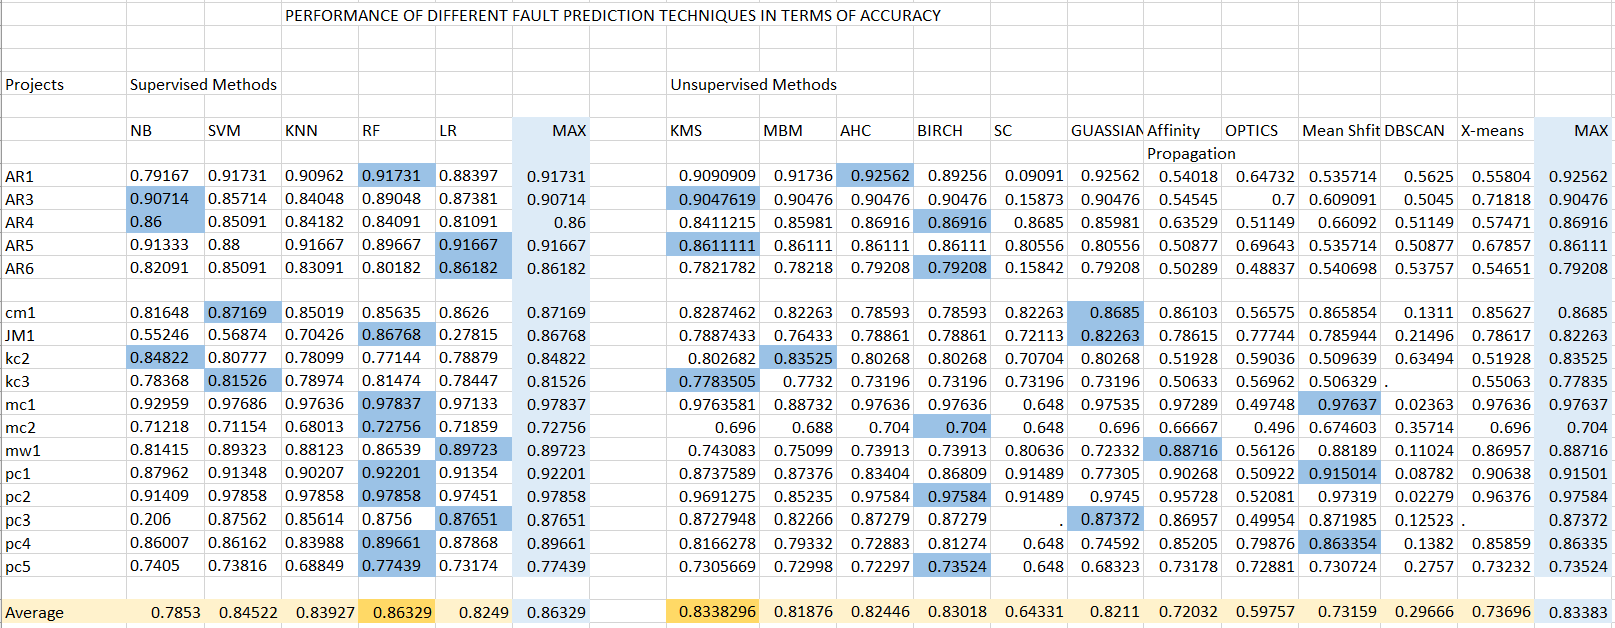
\includegraphics[scale=.6,keepaspectratio=true]{./accuracy}
\end{center}
\begin{table}[]
    \centering
    \caption{Performance of different algorithms in terms of accuracy}
    \label{tab:my_label}
\end{table}

\begin{center}
 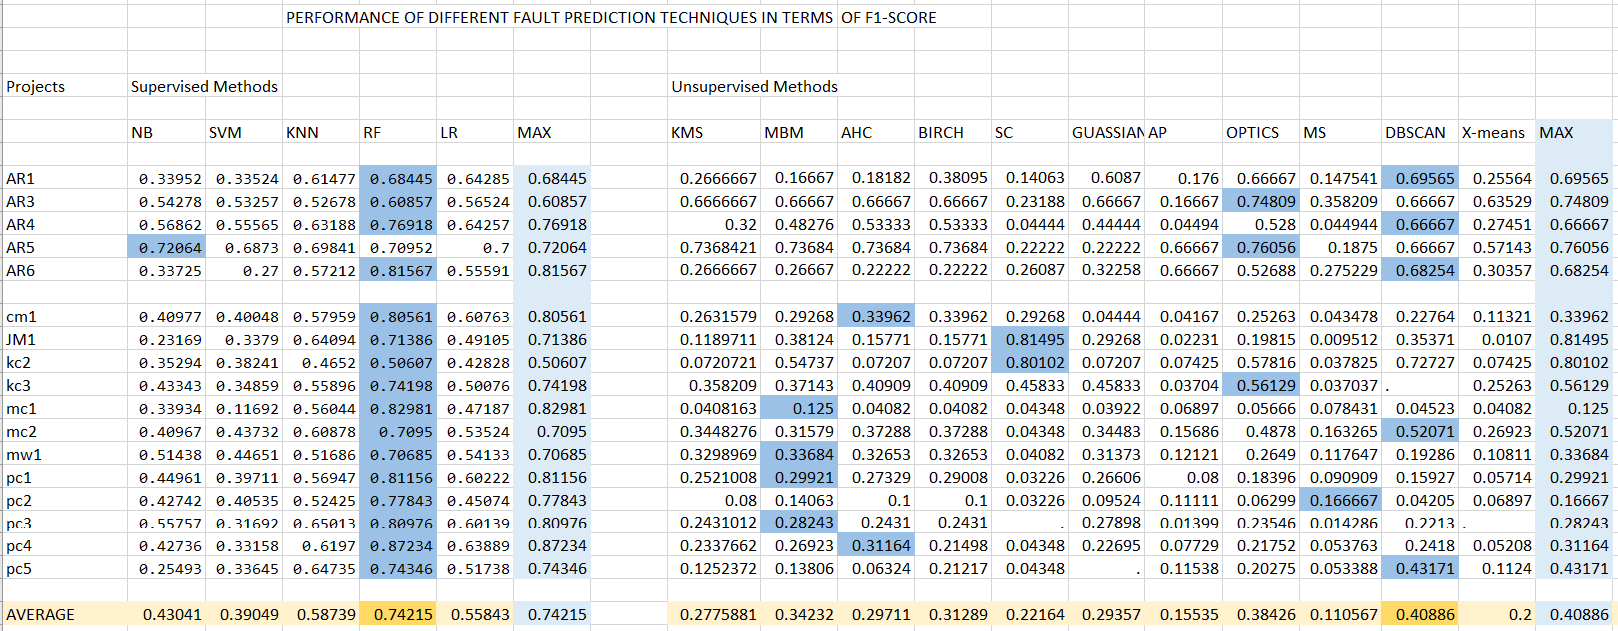
\includegraphics[scale=.5,keepaspectratio=true]{./f1score}
\end{center}
\begin{table}[]
    \centering
    \caption{Performance of different algorithms in terms of f1-score}
    \label{tab:my_label}
\end{table}

\begin{center}
 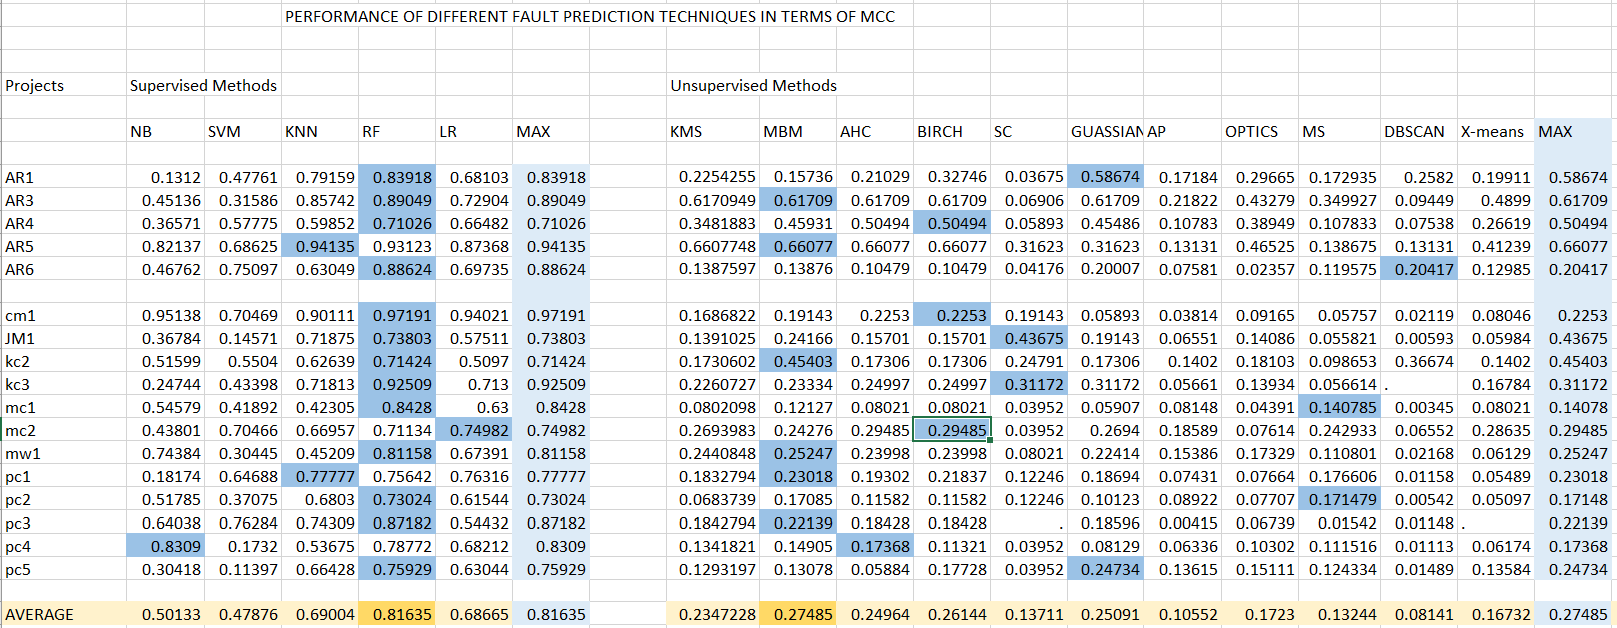
\includegraphics[scale=.5,keepaspectratio=true]{./mcc}
\end{center}
\begin{table}[]
    \centering
    \caption{Performance of different algorithms in terms of MCC}
\end{table}

\pagebreak

\noindent Fig 1 to Fig 17 depict the boxplots of 2 indicators of all supervised models for all 17 datasets.\newline

\begin{figure}[h!]
  \centering
  \begin{subfigure}[b]{0.4\linewidth}
    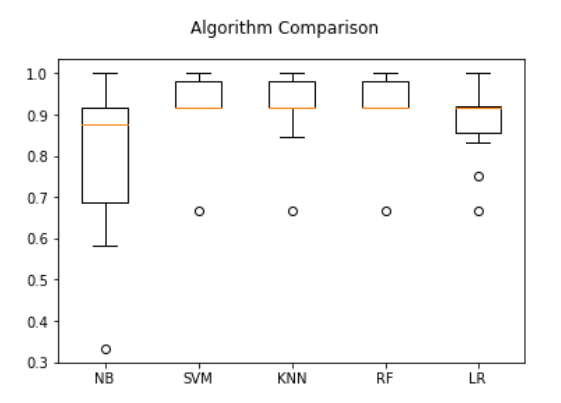
\includegraphics[width=\linewidth]{report/ar1.png}
    \caption{accuracy}
  \end{subfigure}
  \begin{subfigure}[b]{0.4\linewidth}
    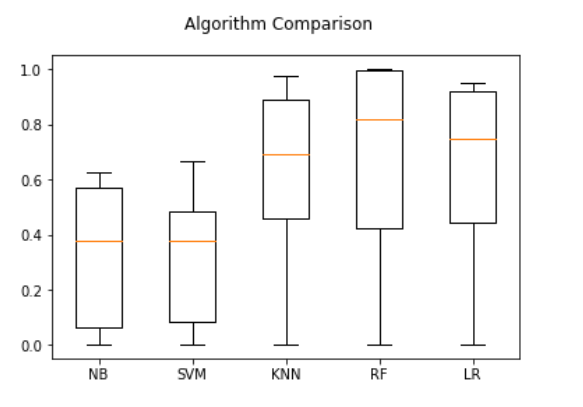
\includegraphics[width=\linewidth]{report/ar1_f.png}
    \caption{f1-score}
  \end{subfigure}
  \caption{Boxplots of supervised models on ar1 dataset}
\end{figure}

\begin{figure}[h!]
  \centering
  \begin{subfigure}[b]{0.4\linewidth}
    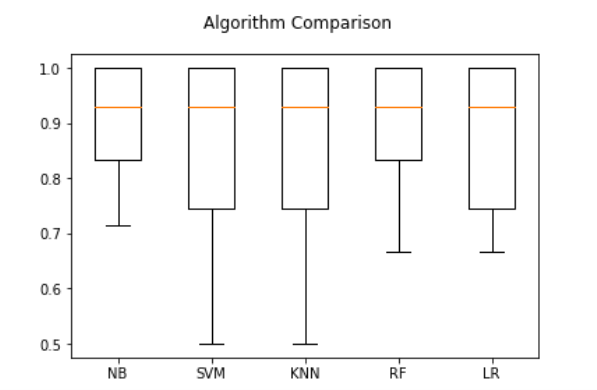
\includegraphics[width=\linewidth]{report/ar3.png}
    \caption{accuracy}
  \end{subfigure}
  \begin{subfigure}[b]{0.4\linewidth}
    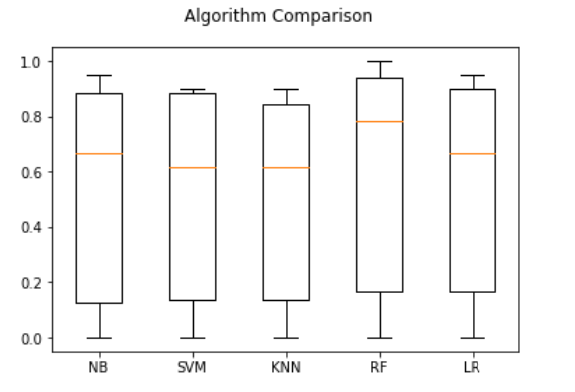
\includegraphics[width=\linewidth]{report/ar3_f.png}
    \caption{f1-score}
  \end{subfigure}
  \caption{Boxplots of supervised models on ar3 dataset}
\end{figure}

\begin{figure}[h!]
  \centering
  \begin{subfigure}[b]{0.4\linewidth}
    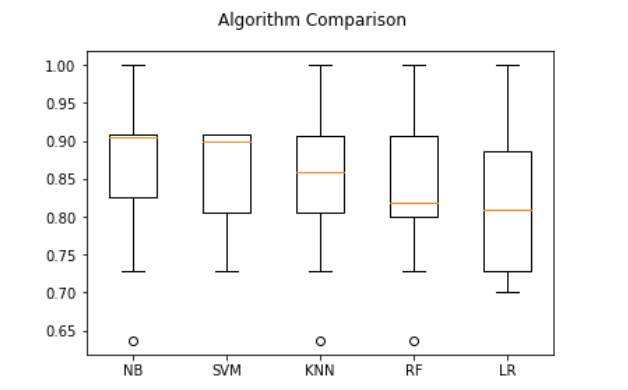
\includegraphics[width=\linewidth]{report/ar4.png}
    \caption{accuracy}
  \end{subfigure}
  \begin{subfigure}[b]{0.4\linewidth}
    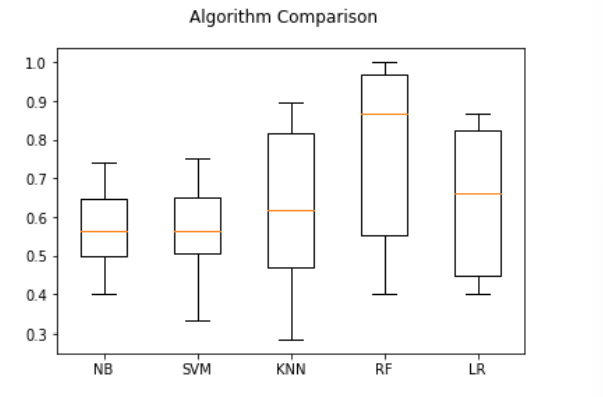
\includegraphics[width=\linewidth]{report/ar4_f.png}
    \caption{f1-score}
  \end{subfigure}
  \caption{Boxplots of supervised models on ar4 dataset}
\end{figure}

\pagebreak

\begin{figure}[h!]
  \centering
  \begin{subfigure}[b]{0.4\linewidth}
    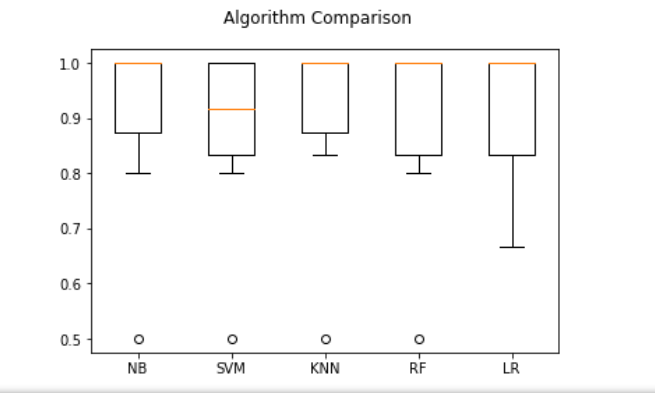
\includegraphics[width=\linewidth]{report/ar5.png}
    \caption{accuracy}
  \end{subfigure}
  \begin{subfigure}[b]{0.4\linewidth}
    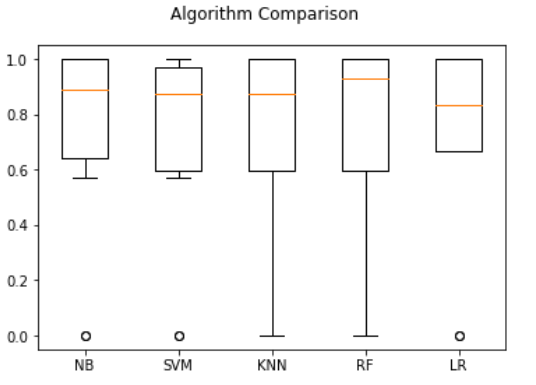
\includegraphics[width=\linewidth]{report/ar5_f.png}
    \caption{f1-score}
  \end{subfigure}
  \caption{Boxplots of supervised models on ar5 dataset}
\end{figure}

\begin{figure}[h!]
  \centering
  \begin{subfigure}[b]{0.4\linewidth}
    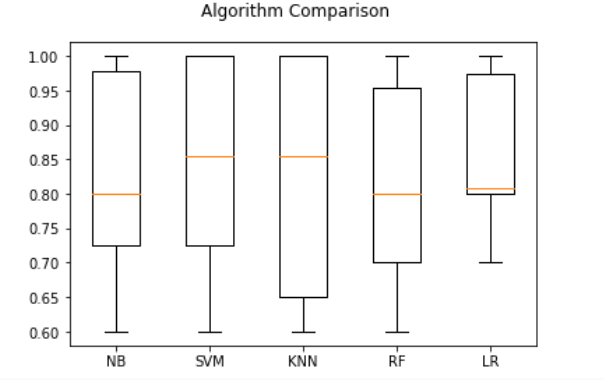
\includegraphics[width=\linewidth]{report/ar6.png}
    \caption{accuracy}
  \end{subfigure}
  \begin{subfigure}[b]{0.4\linewidth}
    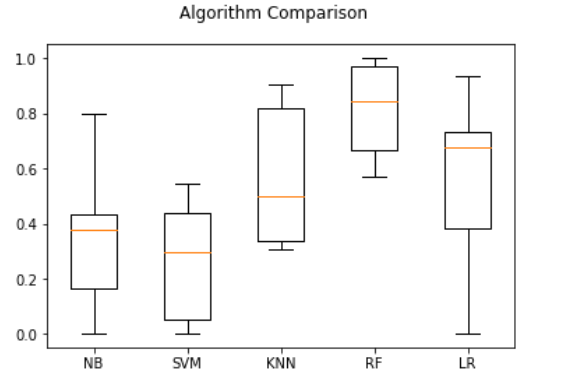
\includegraphics[width=\linewidth]{report/ar6_f.png}
    \caption{f1-score}
  \end{subfigure}
  \caption{Boxplots of supervised models on ar6 dataset}
\end{figure}

\begin{figure}[h!]
  \centering
  \begin{subfigure}[b]{0.4\linewidth}
    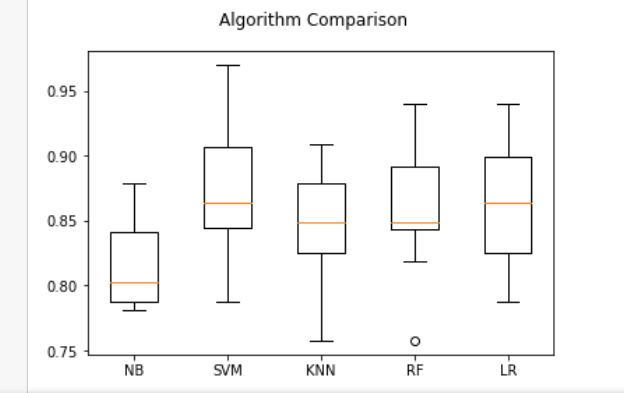
\includegraphics[width=\linewidth]{report/cm1.png}
    \caption{accuracy}
  \end{subfigure}
  \begin{subfigure}[b]{0.4\linewidth}
    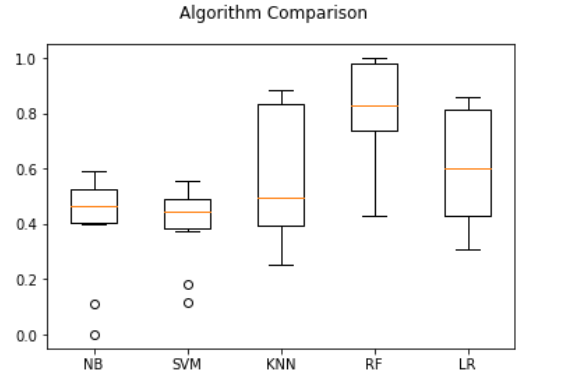
\includegraphics[width=\linewidth]{report/cm1_f.png}
    \caption{f1-score}
  \end{subfigure}
  \caption{Boxplots of supervised models on cm1 dataset}
\end{figure}

\pagebreak

\begin{figure}[h!]
  \centering
  \begin{subfigure}[b]{0.4\linewidth}
    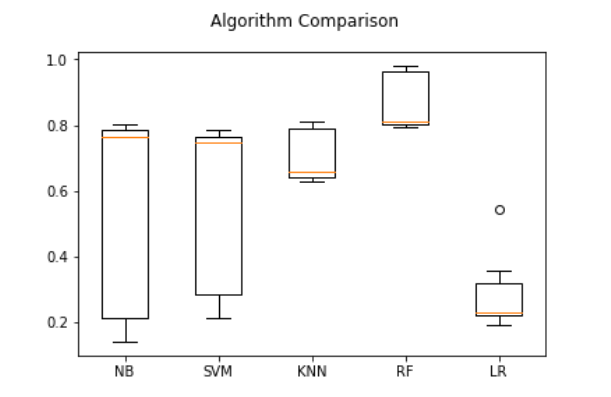
\includegraphics[width=\linewidth]{report/JM1.png}
    \caption{accuracy}
  \end{subfigure}
  \begin{subfigure}[b]{0.4\linewidth}
    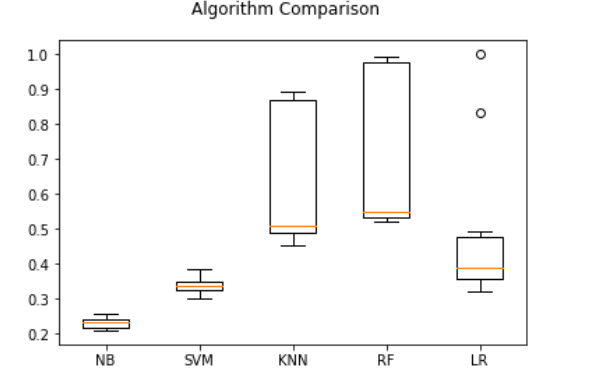
\includegraphics[width=\linewidth]{report/JM1_f.png}
    \caption{f1-score}
  \end{subfigure}
  \caption{Boxplots of supervised models on JM1 dataset}
\end{figure}

\begin{figure}[h!]
  \centering
  \begin{subfigure}[b]{0.4\linewidth}
    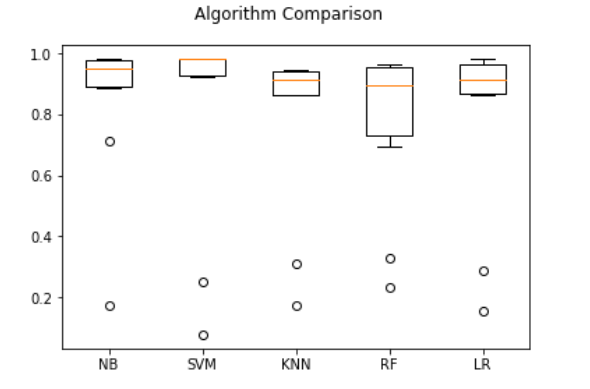
\includegraphics[width=\linewidth]{report/kc2.png}
    \caption{accuracy}
  \end{subfigure}
  \begin{subfigure}[b]{0.4\linewidth}
    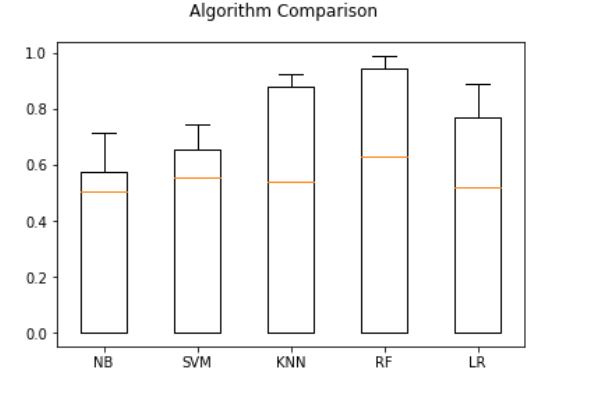
\includegraphics[width=\linewidth]{report/kc2_f.png}
    \caption{f1-score}
  \end{subfigure}
  \caption{Boxplots of supervised models on kc2 dataset}
\end{figure}

\begin{figure}[h!]
  \centering
  \begin{subfigure}[b]{0.4\linewidth}
    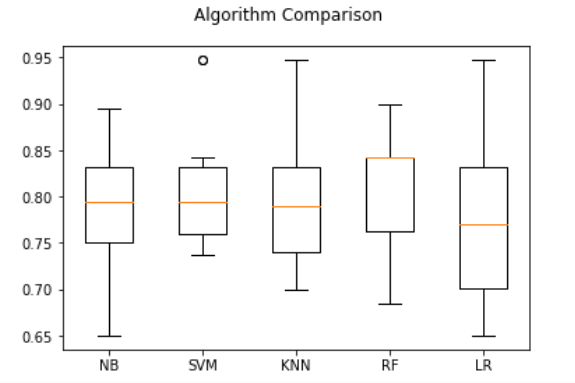
\includegraphics[width=\linewidth]{report/KC3.png}
    \caption{accuracy}
  \end{subfigure}
  \begin{subfigure}[b]{0.4\linewidth}
    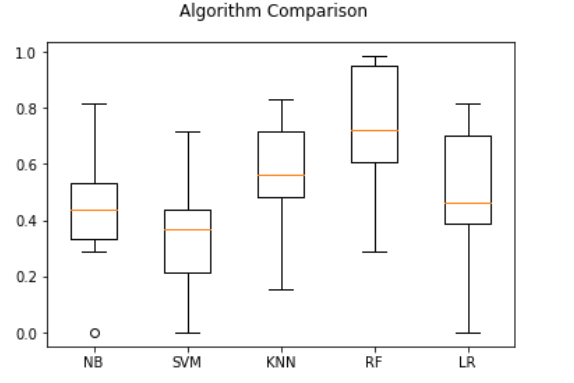
\includegraphics[width=\linewidth]{report/KC3_f.png}
    \caption{f1-score}
  \end{subfigure}
  \caption{Boxplots of supervised models on KC3 dataset}
\end{figure}

\pagebreak

\begin{figure}[h!]
  \centering
  \begin{subfigure}[b]{0.4\linewidth}
    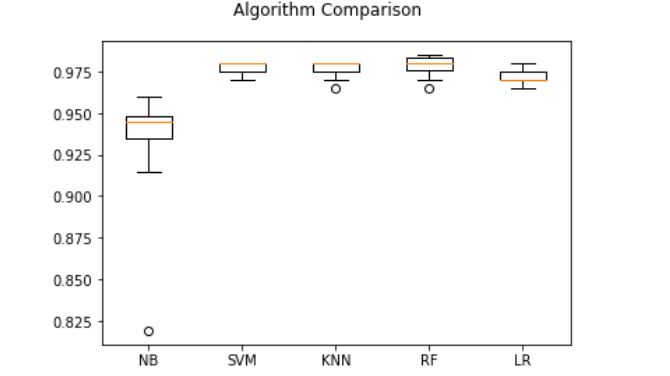
\includegraphics[width=\linewidth]{report/mc1.png}
    \caption{accuracy}
  \end{subfigure}
  \begin{subfigure}[b]{0.4\linewidth}
    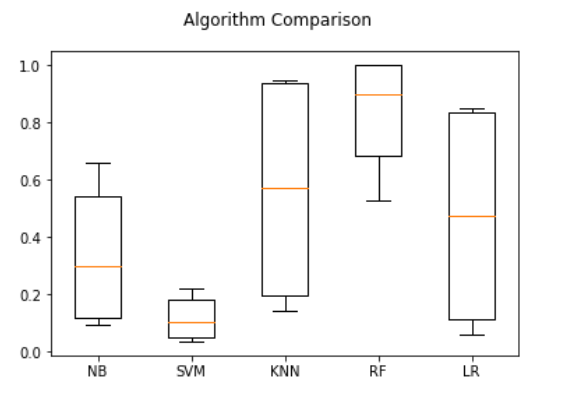
\includegraphics[width=\linewidth]{report/mc1_f.png}
    \caption{f1-score}
  \end{subfigure}
  \caption{Boxplots of supervised models on mc1 dataset}
\end{figure}

\begin{figure}[h!]
  \centering
  \begin{subfigure}[b]{0.4\linewidth}
    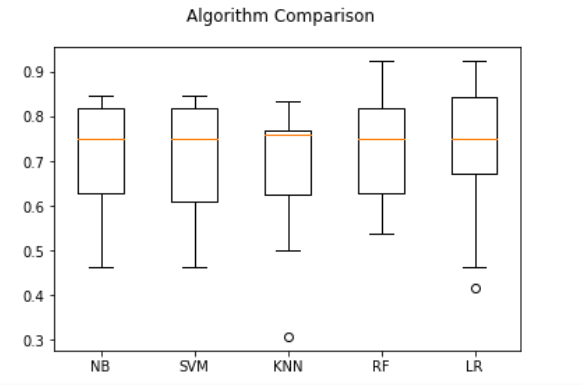
\includegraphics[width=\linewidth]{report/mc2.png}
    \caption{accuracy}
  \end{subfigure}
  \begin{subfigure}[b]{0.4\linewidth}
    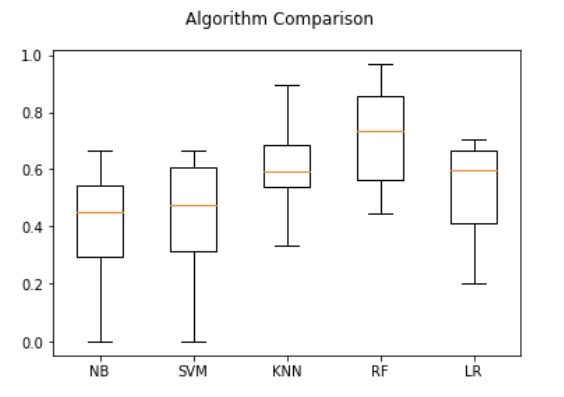
\includegraphics[width=\linewidth]{report/mc2_f.png}
    \caption{f1-score}
  \end{subfigure}
  \caption{Boxplots of supervised models on mc2 dataset}
\end{figure}

\begin{figure}[h!]
  \centering
  \begin{subfigure}[b]{0.4\linewidth}
    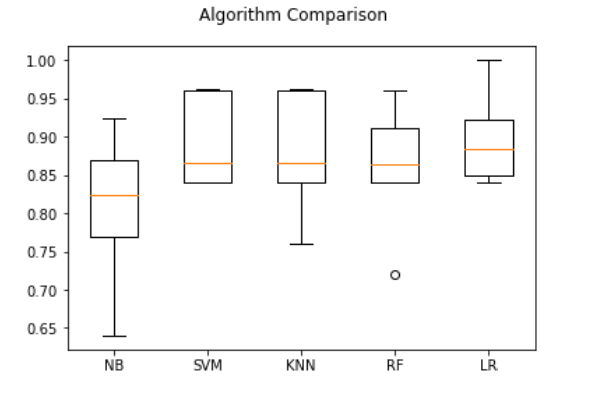
\includegraphics[width=\linewidth]{report/mw1.png}
    \caption{accuracy}
  \end{subfigure}
  \begin{subfigure}[b]{0.4\linewidth}
    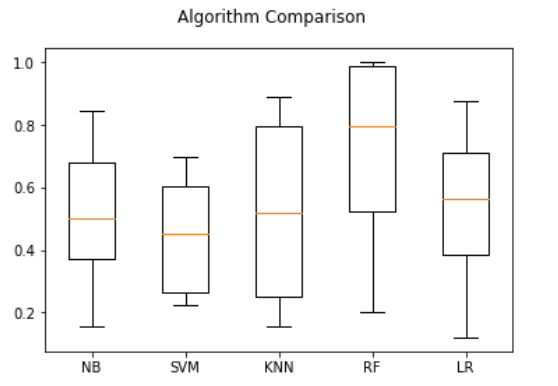
\includegraphics[width=\linewidth]{report/mw1_f.png}
    \caption{f1-score}
  \end{subfigure}
  \caption{Boxplots of supervised models on mw1 dataset}
\end{figure}

\pagebreak

\begin{figure}[h!]
  \centering
  \begin{subfigure}[b]{0.4\linewidth}
    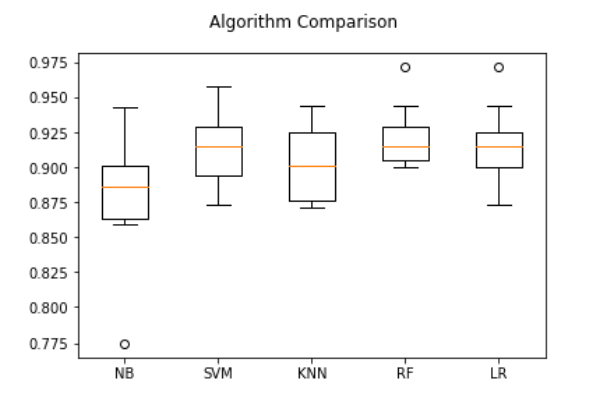
\includegraphics[width=\linewidth]{report/PC1.png}
    \caption{accuracy}
  \end{subfigure}
  \begin{subfigure}[b]{0.4\linewidth}
    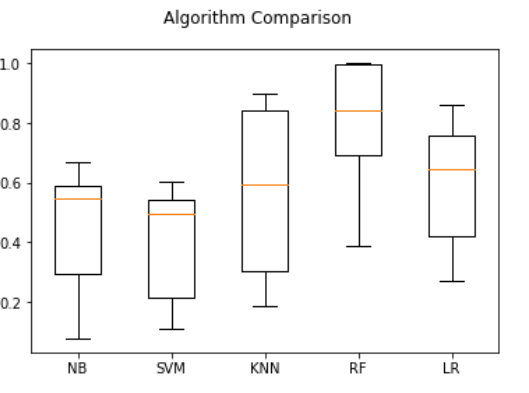
\includegraphics[width=\linewidth]{report/PC1_f.png}
    \caption{f1-score}
  \end{subfigure}
  \caption{Boxplots of supervised models on PC1 dataset}
\end{figure}

\begin{figure}[h!]
  \centering
  \begin{subfigure}[b]{0.4\linewidth}
    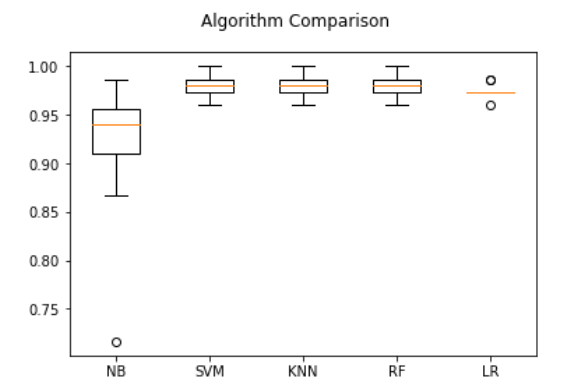
\includegraphics[width=\linewidth]{report/PC2.png}
    \caption{accuracy}
  \end{subfigure}
  \begin{subfigure}[b]{0.4\linewidth}
    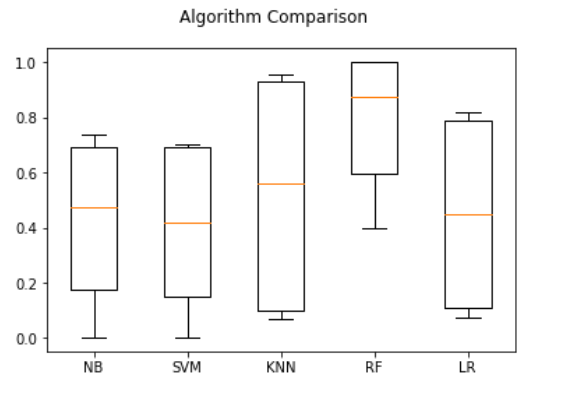
\includegraphics[width=\linewidth]{report/PC2_f.png}
    \caption{f1-score}
  \end{subfigure}
  \caption{Boxplots of supervised models on PC2 dataset}
\end{figure}

\begin{figure}[h!]
  \centering
  \begin{subfigure}[b]{0.4\linewidth}
    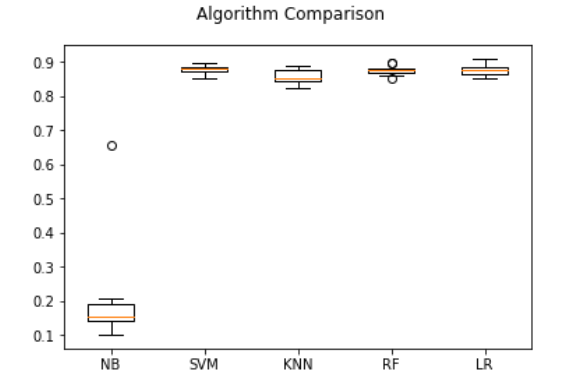
\includegraphics[width=\linewidth]{report/PC3.png}
    \caption{accuracy}
  \end{subfigure}
  \begin{subfigure}[b]{0.4\linewidth}
    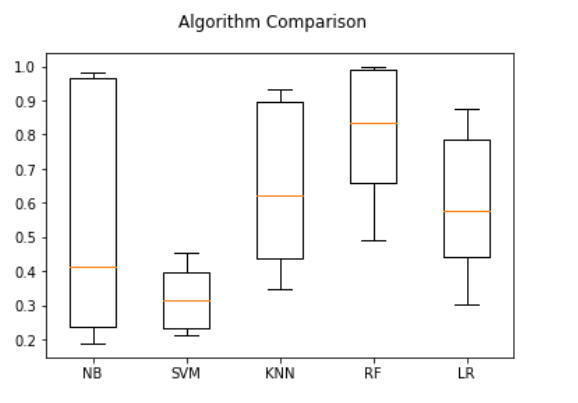
\includegraphics[width=\linewidth]{report/PC3_f.png}
    \caption{f1-score}
  \end{subfigure}
  \caption{Boxplots of supervised models on PC3 dataset}
\end{figure}

\pagebreak

\begin{figure}[h!]
  \centering
  \begin{subfigure}[b]{0.4\linewidth}
    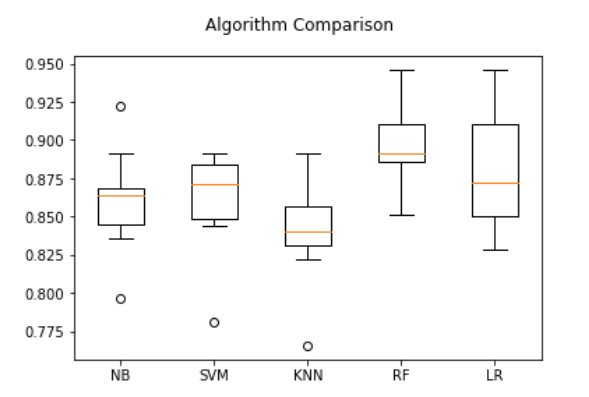
\includegraphics[width=\linewidth]{report/PC4.png}
    \caption{accuracy}
  \end{subfigure}
  \begin{subfigure}[b]{0.4\linewidth}
    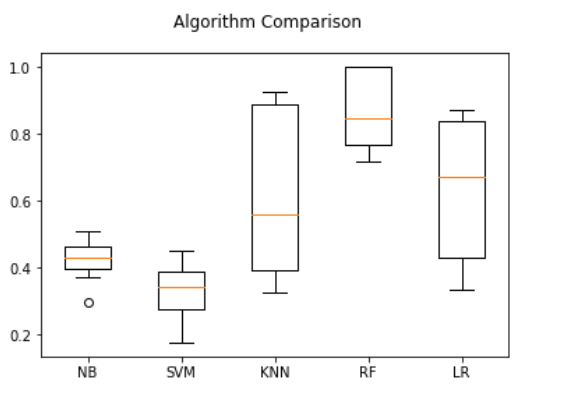
\includegraphics[width=\linewidth]{report/PC4_f.png}
    \caption{f1-score}
  \end{subfigure}
  \caption{Boxplots of supervised models on PC4 dataset}
\end{figure}

\begin{figure}[h!]
  \centering
  \begin{subfigure}[b]{0.4\linewidth}
    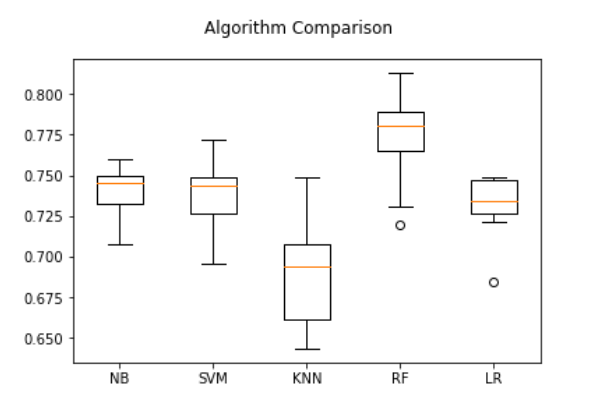
\includegraphics[width=\linewidth]{report/PC5.png}
    \caption{accuracy}
  \end{subfigure}
  \begin{subfigure}[b]{0.4\linewidth}
    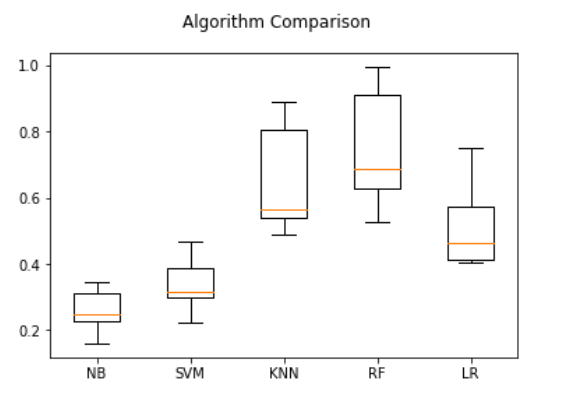
\includegraphics[width=\linewidth]{report/PC5_f.png}
    \caption{f1-score}
  \end{subfigure}
  \caption{Boxplots of supervised models on PC5 dataset}
\end{figure}

\pagebreak

\noindent 1. \underline{In terms of accuracy}\newline
From Table 3.1, we can observe that, for a particular dataset -
In supervised model family except KNN all other models performed well.Also Random Forest (RF) performed best among all other models.In unsupervised models, KMS, BIRCH, Guassian and MS models performed better than other models.\newline
If we talk about average performance of each model over all datasets, Rf is the best model among all supervised clustering models and KMS performed best among all unsupervised models.\newline

\noindent 2. \underline{In terms of f1-score}\newline
From Table 3.2, for a particular dataset, we can say that among all classifiers in the supervised model family RF outperformed other models. Also we can place KNN at second position. In unsupervised model family, MBM, OPTICS and DBSCAN performed better than other models.\newline
If we see average performance of these models, RF is the best model in supervised model family and DBSCAN performed better in unsupervised model family.\newline

\noindent 2. \underline{In terms of MCC}\newline
From Table 3.3, we observe that, for a particular dataset among all classifiers in the supervised model family RF performed best. In unsupervised model family, MBM, BIRCH and Guassian performed better than other models.\newline
If we see average performance of these models, RF is the best model in supervised model family and MBM performed better in unsupervised model family.





